
\subsubsection{5.1 RQ1: Source Identity Produces Large, Statistically Significant Effects (H-E2)}

\textbf{Table 1. HumanEval+ pass@1 by source condition at 1.3B scale (3 seeds)}

\begin{table*}[htbp]
\centering
\resizebox{\dimexpr 2\columnwidth+\columnsep\relax}{!}{%
\begin{tabular}{lllll}
\toprule
Condition & Seed 42 & Seed 123 & Seed 777 & Mean \\
\midrule
HumanEval-only & 39.6\% & 25.6\% & 39.6\% & **35.0\%** \\
MBPP-only & 29.3\% & 27.4\% & 26.2\% & **27.6\%** \\
LeetCode-only & 0.0\% & 0.0\% & 9.1\% & **~3.1\%** \\
Equal-mix & 10.4\% & 9.8\% & 10.4\% & **10.2\%** \\
\bottomrule
\end{tabular}
}
\end{table*}

One-way ANOVA on these 12 observations: F=11.37, p=0.020. Maximum pairwise contrast: HumanEval-only (35.0\%) versus LeetCode-only (~3.1\%) --- a difference of 31.9 percentage points under identical token-budget-equalized, deduplicated, format-normalized conditions.

Equal-mix achieves only 10.2\% --- substantially below both HumanEval-only (35.0\%) and MBPP-only (27.6\%), despite receiving the same effective token budget. Naive multi-source mixing at equal proportions does not outperform focused single-source training on the benchmark most aligned with one of the constituent sources.

LeetCode-only SFT achieves 0.0\% HumanEval+ pass@1 on seeds 42 and 123, with only seed 777 reaching 9.1\%. This high variance across seeds, combined with the near-zero performance, may reflect training instability or sensitivity to initialization for the most distributionally misaligned source condition; training convergence (loss curves) was not separately verified for LeetCode conditions.

The embedding distribution distinctiveness prerequisite (H-E1) was satisfied prior to SFT training. CodeBERT mean pairwise cosine similarities (source $\rightarrow$ test benchmark) ranged from 0.909 (LeetCode $\rightarrow$ HumanEval+) to 0.975 (HumanEval-train $\rightarrow$ HumanEval+); all-MiniLM-L6-v2 similarities ranged from 0.247 (LeetCode $\rightarrow$ MBPP+) to 0.311 (HumanEval-train $\rightarrow$ HumanEval+). All 8 MiniLM source-benchmark pairs fell below the 0.95 distinctiveness threshold.

\begin{figure}[htbp]
\centering
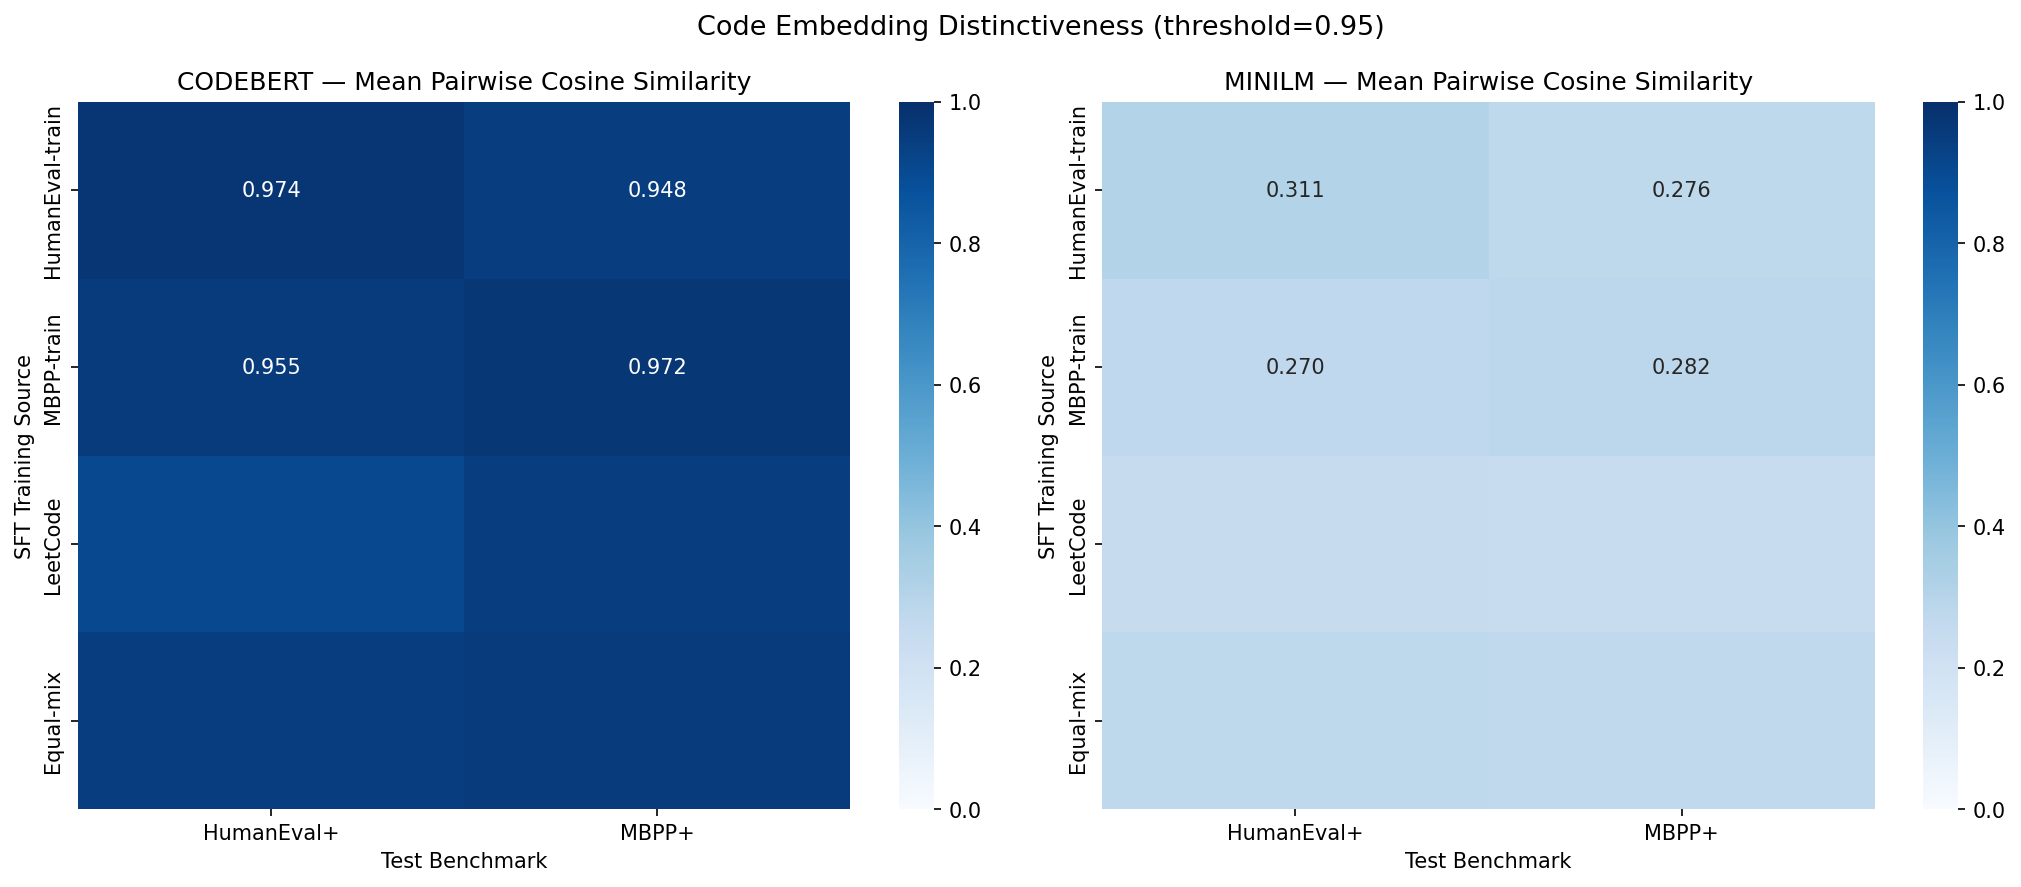
\includegraphics[width=\columnwidth]{figures/similarity_heatmaps.png}
\caption{Figure 1: Dual-encoder similarity matrices}
\label{fig:similarity_heatmaps}
\end{figure}

\textit{Figure 1. CodeBERT (left) and MiniLM (right) mean pairwise cosine similarity between training source corpora (rows) and test benchmarks (columns). MiniLM shows wider separation (0.247--0.311) than CodeBERT (0.909--0.975).}

\subsubsection{5.2 RQ2: Asymmetric, Not Symmetric, Specialization (H-M1)}

The symmetric specialization prediction --- HumanEval-only outperforms MBPP-only on HumanEval+, and MBPP-only outperforms HumanEval-only on MBPP+ --- is not supported. The HumanEval+ direction is partially confirmed (HumanEval-only > MBPP-only in 2/3 seeds); the MBPP+ direction is refuted in all three seeds.

\textbf{Table 2. Per-seed MBPP+ pass@1: HumanEval-only versus MBPP-only (1.3B scale)}

\begin{table}[htbp]
\centering
\resizebox{\columnwidth}{!}{%
\begin{tabular}{llll}
\toprule
Seed & HumanEval-only MBPP+ & MBPP-only MBPP+ & Direction \\
\midrule
42 & 52.4\% & 50.5\% & HE-only higher \\
123 & 51.9\% & 50.3\% & HE-only higher \\
777 & 51.6\% & 50.8\% & HE-only higher \\
\bottomrule
\end{tabular}
}
\end{table}

HumanEval-only training outperforms MBPP-only training on MBPP+'s own benchmark by approximately 1.5--2.1 percentage points consistently across all three seeds. The predicted MBPP+ inversion (MBPP-only > HumanEval-only on MBPP+) is absent.

\textbf{Table 3. Transfer matrix: mean pass@1 across 3 seeds (1.3B scale)}

\begin{table*}[htbp]
\centering
\resizebox{\dimexpr 2\columnwidth+\columnsep\relax}{!}{%
\begin{tabular}{lllll}
\toprule
Benchmark & HumanEval-only & MBPP-only & LeetCode-only & Equal-mix \\
\midrule
HumanEval+ & **35.9\%** & 27.6\% & ~3.1\% & 10.2\% \\
MBPP+ & **51.9\%** & 50.5\% & ~15.6\% & 47.9\% \\
\bottomrule
\end{tabular}
}
\end{table*}

Note: MBPP+ values for LeetCode-only and Equal-mix are reported from H-M1's analysis of H-E2 checkpoints. HumanEval+ values for H-M1 are taken directly from H-M1's scoring (35.9\% for HumanEval-only), which may differ slightly from Table 1 (35.0\%) due to rounding in intermediate computations; both derive from the same three checkpoint evaluations.

\begin{figure}[htbp]
\centering
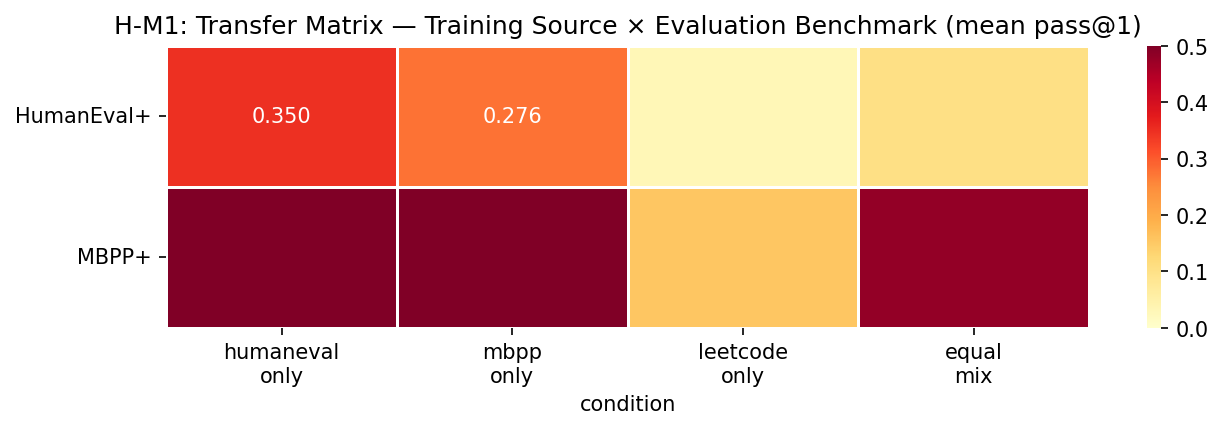
\includegraphics[width=\columnwidth]{figures/heatmap_pass1.png}
\caption{Figure 2: Transfer matrix heatmap}
\label{fig:heatmap_pass1}
\end{figure}

\textit{Figure 2. Mean pass@1 per source condition on both benchmarks (1.3B). HumanEval-only achieves the highest mean pass@1 on both benchmarks.}

\begin{figure}[htbp]
\centering
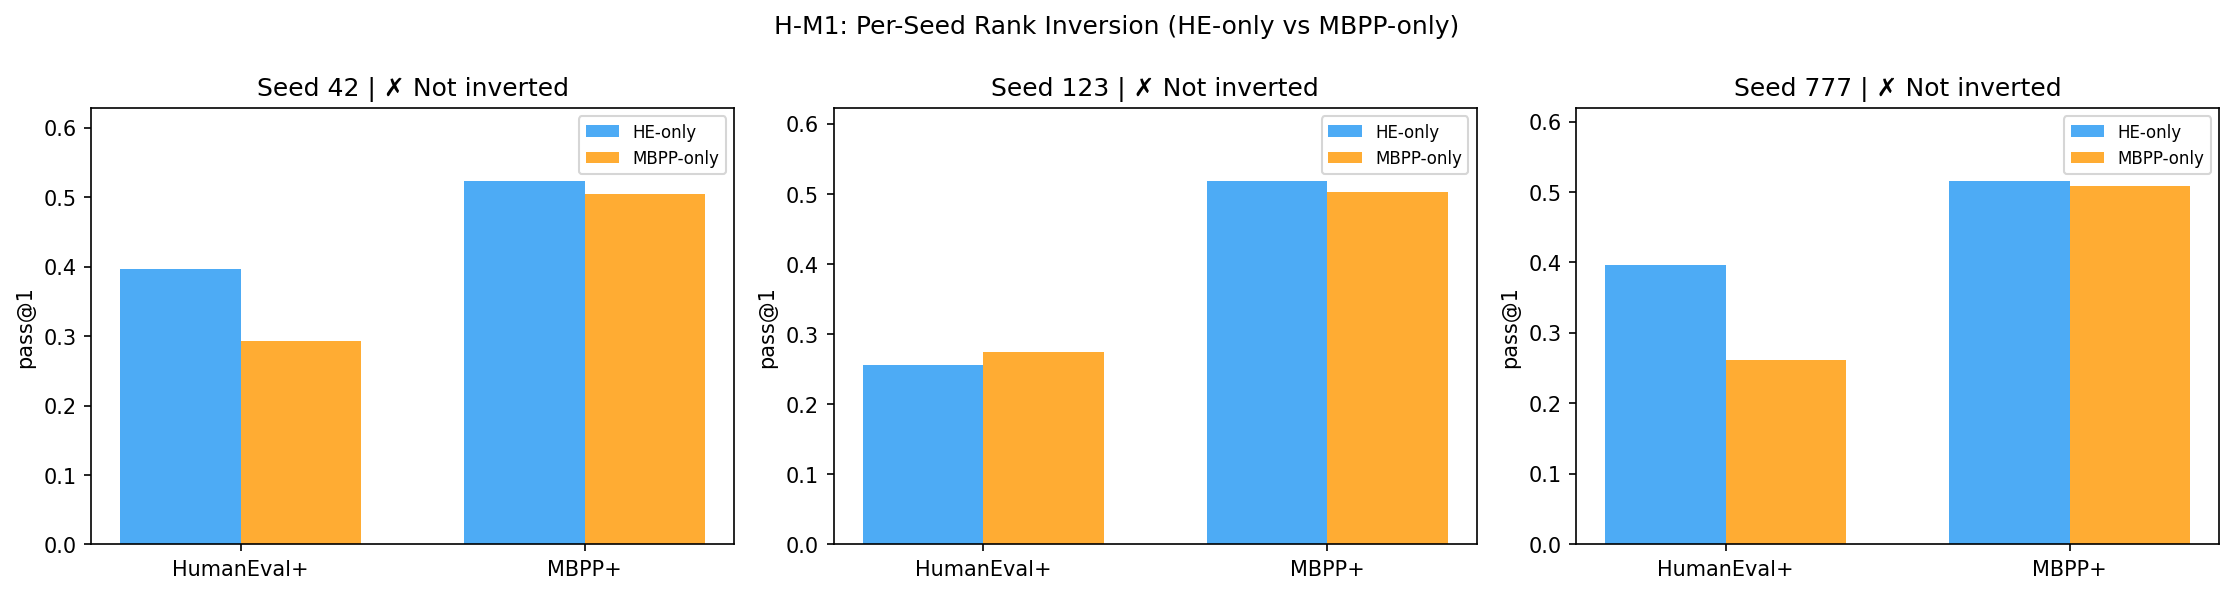
\includegraphics[width=\columnwidth]{figures/per_seed_inversion.png}
\caption{Figure 3: Per-seed inversion plot}
\label{fig:per_seed_inversion}
\end{figure}

\textit{Figure 3. Per-seed pass@1 for HumanEval-only and MBPP-only on HumanEval+ and MBPP+. The expected MBPP+ inversion (MBPP-only higher than HumanEval-only on MBPP+) is absent in all three seeds.}

\subsubsection{5.3 RQ3: Embedding Alignment Predicts Performance Rank (H-M2)}

\textbf{Table 4. CodeBERT embedding similarity rank versus HumanEval+ pass@1 rank (1.3B)}

\begin{table*}[htbp]
\centering
\resizebox{\dimexpr 2\columnwidth+\columnsep\relax}{!}{%
\begin{tabular}{lllll}
\toprule
Condition & CodeBERT sim to HE+ & Similarity rank & HE+ mean pass@1 & Pass@1 rank \\
\midrule
HumanEval-only & 0.9745 & 1 & 35.0\% & 1 \\
MBPP-only & 0.9547 & 2 & 27.6\% & 2 \\
Equal-mix & 0.9459 & 3 & 10.2\% & 3 \\
LeetCode-only & 0.9091 & 4 & ~3.1\% & 4 \\
\bottomrule
\end{tabular}
}
\end{table*}

Spearman $\rho$ = 1.000; permutation test p = 0.0417 (n=10,000 shuffles, one-sided, \texttt{permutation\textbackslash \_type='pairings'}). Bootstrap 95\% CI: [1.000, 1.000]. MiniLM encoder: $\rho$ = 0.800, p = 0.167 (not significant independently, but direction concordant with CodeBERT).

With n=4 conditions, the minimum achievable permutation p-value is 1/24 $\approx$ 0.042. The observed $\rho$=1.0 achieves exactly this minimum. This means that one rank transposition in the alignment or pass@1 ordering would lose statistical significance. This fragility at n=4 is a structural limitation of the experiment design, not an artifact of the analysis. The finding should be interpreted as ''highly consistent with'' the distributional alignment mechanism rather than as definitive confirmation.

Dual-encoder concordance --- both CodeBERT and MiniLM showing $\rho$ > 0 on HumanEval+ --- is satisfied. MBPP+ alignment rank analysis cannot be conducted: H-E2's CSV output contains only HumanEval benchmark rows; MBPP+ pass@1 data for all four conditions was not saved, making the MBPP+ cells untestable.

\begin{figure}[htbp]
\centering
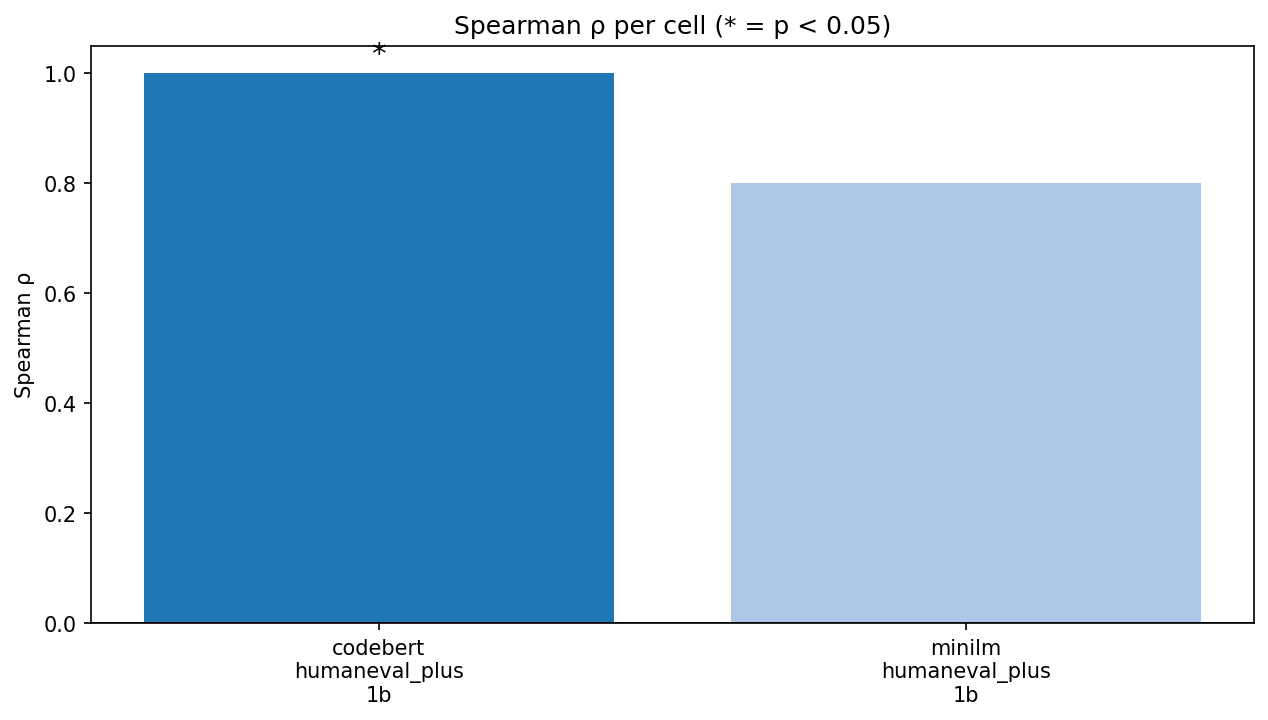
\includegraphics[width=\columnwidth]{figures/fig1_rho_bar_chart.png}
\caption{Figure 4: Spearman $\rho$ bar chart}
\label{fig:fig1_rho_bar_chart}
\end{figure}

\textit{Figure 4. Spearman $\rho$ per encoder for HumanEval+ at 1.3B. CodeBERT achieves $\rho$=1.0 (p=0.042); MiniLM achieves $\rho$=0.80 in the same direction (p=0.167).}

\begin{figure}[htbp]
\centering
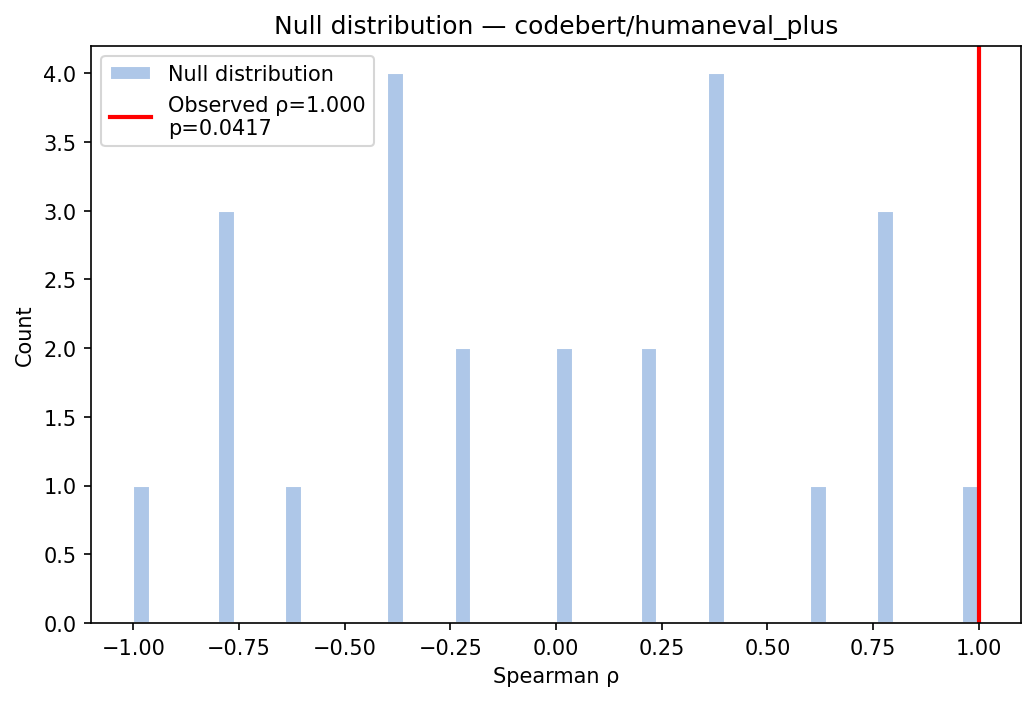
\includegraphics[width=\columnwidth]{figures/fig3_null_distribution.png}
\caption{Figure 5: Permutation null distribution}
\label{fig:fig3_null_distribution}
\end{figure}

\textit{Figure 5. Permutation null distribution (n=10,000) for the CodeBERT / HumanEval+ cell. The observed $\rho$=1.0 falls at p=0.042.}

\subsubsection{5.4 RQ4: Scale Preserves Rank Order with Reduced Magnitude (H-C1)}

\textbf{Table 5. HumanEval+ pass@1 at 7B scale (DeepSeek-Coder-7B-Base, 3 seeds)}

\begin{table*}[htbp]
\centering
\resizebox{\dimexpr 2\columnwidth+\columnsep\relax}{!}{%
\begin{tabular}{lllll}
\toprule
Condition & Seed 42 & Seed 123 & Seed 777 & Mean \\
\midrule
HumanEval-only & 38.4\% & 39.0\% & 38.4\% & **38.6\%** \\
MBPP-only & 37.8\% & 36.6\% & 37.8\% & **37.4\%** \\
LeetCode-only & 34.1\% & 34.1\% & 34.1\% & **34.1\%** \\
Equal-mix & 39.6\% & 39.6\% & 39.6\% & **39.6\%** \\
\bottomrule
\end{tabular}
}
\end{table*}

Absolute condition spread at 7B: 39.6\% $-$ 34.1\% = \textbf{5.5pp} versus 35.0\% $-$ 3.1\% = \textbf{31.9pp} at 1.3B. The rank order changes at 7B: Equal-mix (39.6\%) rises to match or exceed HumanEval-only (38.6\%), suggesting that larger pretraining scale reduces the penalty for distributional diversity during SFT.

Within-condition seed variance: $\sigma ^2 \approx$ 0.00043 at 7B versus $\sigma ^2 \approx$ 0.01655 at 1.3B. At 7B, each condition produces near-identical scores across seeds (e.g., LeetCode-only yields 34.1\% on all three seeds).

\textbf{On the $\eta^2$ comparison:} $\eta^{2}_7B$ = 0.977 exceeds $\eta^{2}_{1}.3B$ = 0.912 despite a smaller absolute spread at 7B. This occurs because $\eta^2$ = SS\_between / SS\_total; when within-condition variance collapses to near-zero (as at 7B), $\eta^2$ inflates mechanically regardless of the actual between-condition effect size. Absolute condition spread is the appropriate metric for comparing source identity effect magnitude across scales.

MBPP+ evaluation at 7B is incomplete: 4 of 12 evaluations failed with parse errors due to tokenizer incompatibility. A post-hoc patch was applied, but MBPP+ results were not recovered within the experiment window.

\begin{figure}[htbp]
\centering
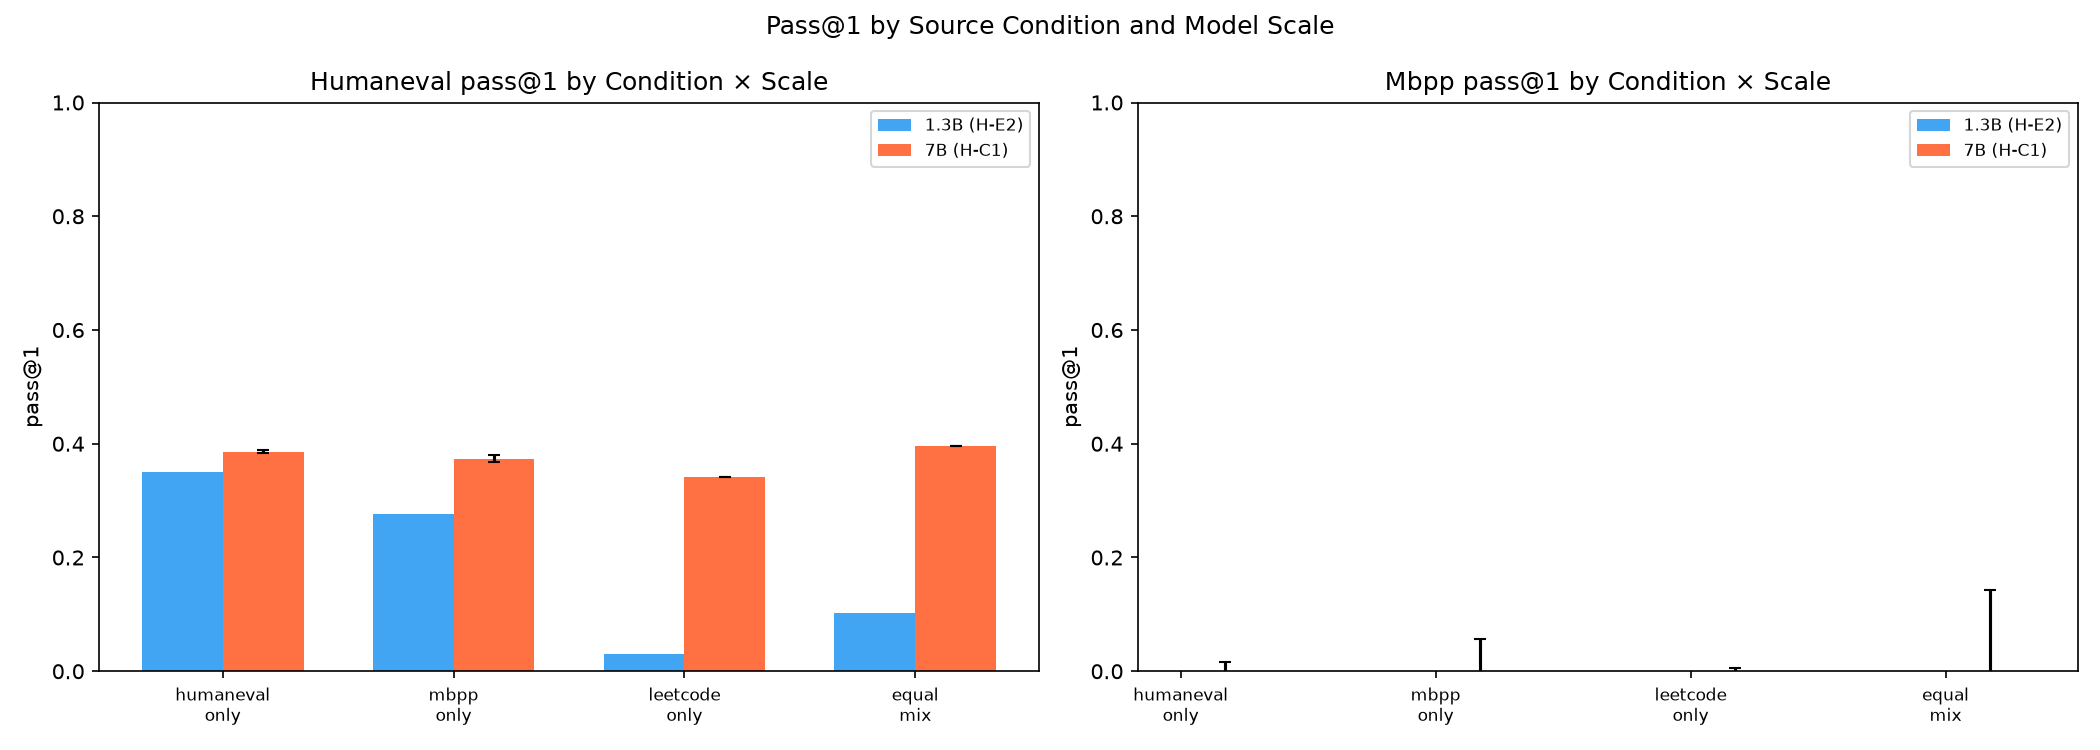
\includegraphics[width=\columnwidth]{figures/pass1_by_condition_scale.png}
\caption{Figure 6: Pass@1 by condition and scale}
\label{fig:pass1_by_condition_scale}
\end{figure}

\textit{Figure 6. HumanEval+ pass@1 by SFT condition at 1.3B and 7B scale. Absolute spread narrows from 31.9pp to 5.5pp; Equal-mix rises relative to HumanEval-only at 7B.}

